This chapter is very technical and should give a walk through the chosen technology, show the architecture, frame the implementation effort, and explain the taken decisions while working on this thesis.

First we will introduce the different technologies and how they play together. Second we will shortly define the frames of reference and the architecture of the implementation. Then the particle filter implementation will be explained in detail and how the filter routine works and from what parameters we can choose from. Afterwards a few intermediate steps and solved issues that should come up while working on this thesis are discussed. At the end the platform implementation in case of Android and the effort made on visualization is described.

\section{Technology}

The major criteria for the choice of technology was platform independence and real-time processing. Platform independence because there are two different mobile user platforms with Android and iOS and the need of an evaluation framework that runs on a desktop environment like Ubuntu. Since this calibration is online, real-time processing is necessary and therefore there is a critical performance limit attached. When one seconds of real-time has passed we have to process at least one second of sensor data.

Similar to the algorithm, the visualization was planned to be platform independent with the benefit that it could be displayed on the smartphone and on the desktop for evaluation purposes. The first attempt was to use OpenGL from C++ but that would have brought a lot of overhead to the implementation. Since all target platforms have an HTML5 compatible browser the final attempt was to use JavaScript for that purpose. To communicate with C++ in real-time, WebSocket was used to exchange Protocol Buffers.

Besides the implementation of the algorithm a small Android application was developed in Java which is responsible for reading the sensors and providing a small user interface.

Table \ref{tbl:code_lines} gives a quick overview about the used languages and the implementation effort by lines of code.

\begin{table}[h]
    \centering
    \begin{tabular}{ | l | r | }
    \hline
    \textbf{Language} & \textbf{Total lines of code} \\ \hline
    C++               & 3092 \\ \hline
    Java              &  366 \\ \hline
    JavaScript        &  450 \\ \hline
    Python            &  179 \\ \hline
    Protocol Buffers  &   55 \\ \hline
    CMake             &  203 \\ \hline
    \end{tabular}
    \caption{Total lines of code by language written for this thesis.}
    \label{tbl:code_lines}
\end{table}

\subsection{C++}

The major programming language used in this project is C++ for various reasons. Since C++11 there is a sufficient standard library for common data structures, random variables and common algorithms. C++ is platform independent and can reach major smartphone platforms like Android and iOS. Performance was critical for the implementation which is is a major purpose of C++. Besides that C++ is a modern programming language with multiple paradigms for example it is object-oriented and generic.

Along with C++ multiple tools, frameworks, and libraries were used which are shortly described in the following.
\begin{itemize}
  \item \textbf{boost} is a popular C++ library that comes in handy where the standard library is missing functionality. this thesis only depends on \textbf{boost asio} for networking and \textbf{boost beast} for HTTP and WebSocket.
  \item \textbf{Eigen} is a rich library for linear algebra and comes with implementations for matrices, vector, and quaternions.
  \item \textbf{gtest} is a unit test framework from Google and was used to write small self-contained (unit) test cases.
  \item \textbf{CMake} was used as dependency management and build system.
\end{itemize}

\subsection{Android}

Android is a mobile operating system based on a modified version of the Linux kernel and other open source software. It is primarily designed for mobile devices with touchscreen such as smartphones and tablets. Android is developed by a consortium of developers known as the Open Handset Alliance and commercially sponsored by Google. It was unveiled in November 2007, with the first commercial Android device launched in September 2008.

Android has been the best-selling OS worldwide on smartphones since 2011 and on tablets since 2013. As of May 2017, it has over two billion monthly active users, the largest installed base of any operating system.

Android is one of the target platforms for this thesis. Native applications can be developed with Android Studio in Java or Kotlin. Apart from that, C++ can be integrated and called through \gls{jni} for shared libraries access, low-level and high performance applications.

\subsection{JavaScript}

JavaScript was used to achieve platform independent visualization that can be displayed on desktop and mobile devices. In contrast to the original approach via OpenGL it was more straight forward to use with \textbf{plotly} and a \textbf{matplotlib} background in Python. Additionally, modern browsers come with a WebSocket implementation which reduced the complexity of communication to C++ code.

Along with JavaScript multiple tools, frameworks, and libraries were used which are shortly described in the following.
\begin{itemize}
  \item \textbf{webpack} is a module bundler. Its main purpose is to bundle JavaScript files for usage in a browser.
  \item \textbf{plotly} is a rich plotting library for JavaScript and Python and was used for visualization purposes.
  \item \textbf{THREE} is a library for linear algebra and comes with implementations for matrices, vector, and quaternions.
\end{itemize}

\subsection{Protocol Buffers}

Protocol Buffers (short Protobuf) are Google's language-neutral, platform-neutral, extensible mechanism for serializing structured data. It is useful for programs which communicate with each other over a wire or for storing data. Protocol Buffers has an interface description language that defines the structure of the data and comes with a program that generates source code from that definition that deals with generating or parsing streams of bytes that represents the structured data. The data is serialized in binary representation which takes up less space compared to a text representation like JSON and therefore needs less bandwith while communicating over network.

\section{Frame of reference}
% quaternion transforms from what to what?
% TODO ref images https://developer.android.com/reference/android/hardware/SensorEvent

An important choice while dealing with sensors that have spatial orientation is the frame of reference. Two frames had to be chosen: one for the phone and its sensors and one global. The chosen axis align with those defined in the Android sensor SDK and are shown in Figure \ref{fig:coords}. While magnetic field sensor readings are taken in the phone's frame of reference it is important to transform those measurements to the global frame of reference since there the magnetic field is expected to be constant in close proximity.

The transformation between those two frames is estimated based on the accelerometer and gyroscope. These two sensors can be fused together to form an \gls{imu}. While the accelerometer provides information about two rotation angles, the gyroscope can be used to make the estimate more reliable while the phone is in motion and therefore in acceleration and it can give an relative estimate about the horizontal orientation between two points in time which will drift due to measurement errors.

% TODO full name / reference paper / algorithm name
In this thesis an algorithm designed by Madgwick was used to estimate the orientation of the phone. See Section \ref{sec:ori_est} for further details.

\begin{figure}[hbt!]
    \centering
    \begin{subfigure}{0.4\textwidth}
        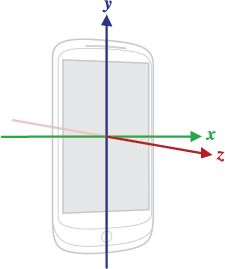
\includegraphics[height=1.0\linewidth]{figures/coords_phone.png}
    \end{subfigure}
    \begin{subfigure}{0.4\textwidth}
        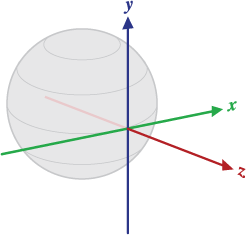
\includegraphics[height=1.0\linewidth]{figures/coords_global.png}
    \end{subfigure}
    \caption{Chosen frames of reference. Gracefully taken from Android sensor SDK documentation.\cite{android_sdk_sensorevent}}
    \label{fig:coords}
\end{figure}

\section{Architecture}

Since the implementation was growing fast in complexity it was important to structure the project into logical and modular components. A lot of thoughts went into code architecture and design decisions which will be shortly discussed here.

The desired architecture had to deal with multiple programming languages and potential concurrency issues. Apart from that, algorithms should be modules that only depend on their input and output which makes it easy to swap them and to test them in a generalized way. Another possible advantage could be the ability to systematically detect bottle necks.

The different algorithms ended up as plugable components in a pipelining scheme. Sensor and filtered data is passed through pipes from node to node. The architecture was applied to the C++ code and the messaging protocol defined with Protocol Buffers. It was also applied in JavaScript but in a more simplified fashion. On Android, Java was used to call \gls{jni} wrapper functions to C++ and therefore did not require any particular architecture.

\begin{figure}[hbt!]
    \centering
    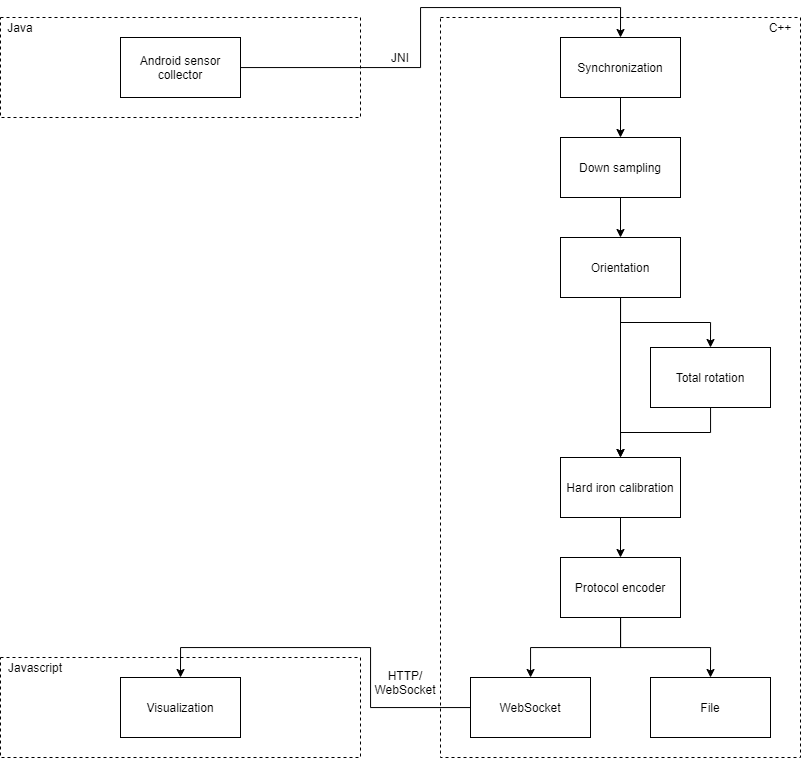
\includegraphics[width=1.0\textwidth]{figures/architecture.png}
    \caption{Architecture of the implementation.}
    \label{fig:architecture}
\end{figure}

\section{Particle filter}
\label{sec:impl_pf}

% TODO shortly walk through the subsections

The bootstrap filter (or sampling importance resampling filter) was chosen as a template for the following implementation.\cite{Kuensch2013}\cite{Doucet2011}

Initially the particle filter was designed to model the full decomposition given by \ref{eq:decomposition}. Since $\bm{B}_{earth}$ and $\bm{B}_{env}$ transform the same way under rotation of the device and we do not have a model for $\bm{B}_{env}$ this approach failed and the particle filter was further simplified.

\subsection{Likelihood}

In Bayesian statistics, likelihood is the key to model an update from a prior to a posteriori distribution. Since we do this numerically we have to be careful with the numerical limitations of our underlying machine. We expect single-precision floating-points as IEEE 754-1985 with the following properties: 1 sign bit, 8 exponent bits, 23 significant precision bits. This leads to an exponent range of $[-126,127]$. Since likelihood arithmetic involves multiplications on very small numbers we have to use the log likelihood instead.

To calculate the weights from the log likelihood we used the largest log likelihood involved and subtract it. This is possible because the weights are invariant under scalar multiplication and can be renormalized if necessary. It also maps the weights to numbers in the range $[0, 1]$.

\subsection{One particle}

One particle represents the state of one realization of the hard iron calibration. The calibration can be parameterized with a three dimensional vector representing the offset of the measurement to the true value. Another vector keeps the estimated external field which is $\bm{B}_{external} = \bm{B}_{measure} - \bm{B}_{phone}$ with $\bm{B}_{phone}$ as the hard iron offset. The external field can later be compared to the next estimate to see if is consistent. At last, we also store the \textit{log likelihood} $\ell$ and \textit{weight} $\mathcal{W}$. They are related to each other but it was handy to keep them separate and might have performance advantages we do not need to convert between them all the time.

\begin{table}[h]
    \centering
    \begin{tabular}{ | l | p{10cm} | }
    \hline
    \textbf{Field}             & \textbf{Description} \\ \hline
    \textsc{hardIron}          & The hard iron offset represented by this particle. \\ \hline
    \textsc{external}          & The external magnetic field $\bm{B}_{external}$ consistent with the last measurement. \\ \hline
    \textsc{logLikelihood}     & Logarithm of the likelihood of this particle $\ell$. \\ \hline
    \textsc{weight}            & The weight $\mathcal{W}$ describes how likely this realization is. It is a relative measure to the total weight among all particles. \\ \hline
    \end{tabular}
    \caption{Description of the properties of one particle.}
    \label{tbl:one_particle}
\end{table}

\subsection{Initialization}

At the very first the particle filter has to be initialized with an a priori distribution for the hard iron calibration. Without taking further assumptions a Gaussian distribution $N(0, \sigma^2)$ was chosen to sample each component of the hard iron vector. To be consistent with the external magnetic field $\bm{B}_{external}$ property of the particles we also need an initial magnetometer observation.

If the device was calibrated in the past we could choose that as the center of our distribution or use a mixture with one at the origin. The calibration of the operating system might also be a reasonable starting point of our calibration.

Pseudocode can be found in Algorithm \ref{alg:pf_init}.

\begin{algorithm}[h]
	\KwIn{population size $n$, hard iron variance $\sigma^2$, magnetic field measurement $\bm{B}_{measure}$, orientation $\bm{q}$}
	\KwOut{initialized and populated particle filter $P$}
	$P \leftarrow$ \textsc{allocateParticles}($n$)\\
	\ForEach{particle in $P$}{
		$\bm{B}_{phone} \leftarrow$ \textsc{gaussianDrawThree}($0$, $\sigma^2$)\\
		\smallskip
		$\bm{B}_{external} \leftarrow q \times (\bm{B}_{measure} - \bm{B}_{phone})$\\
		\smallskip
		$\ell \leftarrow -\log{n}$\\
		\smallskip
		$\mathcal{W} \leftarrow \frac{1}{n}$\\
	}
	\Return{$P$}
	\caption{Initialization of the particle filter as pseudocode.}
	\label{alg:pf_init}
\end{algorithm}

\subsection{Propagation}

In order to propagate our particles we have to apply a state transition. Since we do not have a physical model of how the hard iron effect will evolve over time the idea was to apply a random walk for each particle. That approach allows the particle filter to do recalibration over time and simplifies the reampling step.

Pseudocode can be found in Algorithm \ref{alg:pf_prop}.

\begin{algorithm}[h]
	\KwIn{population $P$, time passed $t$, hard iron variance drift rate $\sigma^2$}
	\KwOut{population $P$}
	\ForEach{particle in $P$}{
		$\bm{B}_{phone} \leftarrow \bm{B}_{phone}$ + \textsc{gaussianDrawThree}($0$, $t * \sigma^2$)\\
	}
	\Return{$P$}
	\caption{Propagation step of the particle filter as pseudocode.}
	\label{alg:pf_prop}
\end{algorithm}

\subsection{Update}

We update our particle filter by offering new observations from the magnetometer and orientation filter. The orientation is used to transform the magnetic field into the local frame of reference of the device. From transformed measurement we can subtract the hard iron vector and get the external field $\bm{B}_{external} = \bm{B}_{measure} - \bm{B}_{phone}$. Based on the estimated external field and the previous result the likelihood can be calculated which was modeled by a Gaussian distribution $N(0, \sigma^2)$. $\sigma^2$ can be used to parameterize the noise of the sensor and the variation of the magnetic field between two different points in space.

Pseudocode can be found in Algorithm \ref{alg:pf_update}.

\begin{algorithm}[h]
	\KwIn{population $P$, magnetic field measurement $\bm{B}_{measure}$, orientation $q$, prediction variance $\sigma^2$}
	\KwOut{population $P$}
	\ForEach{particle in $P$}{
	    $\bm{B}_{prediction} \leftarrow \bm{B}_{phone} + q^{-1} \times \bm{B}_{external}$\\
	    $\ell \leftarrow \ell +$ \textsc{gaussianLogPDF}($\bm{B}_{external}$, $\bm{B}_{prediction}$, $\sigma^2$)\\
	    $\bm{B}_{external} \leftarrow q \times (\bm{B}_{measure} - \bm{B}_{phone})$\\
	}
	\Return{$P$}
	\caption{Update step of the particle filter as pseudocode.}
	\label{alg:pf_update}
\end{algorithm}

\subsection{Resampling}

The resampling step is the most important part of the particle filter. Without it the likelihood would converge to zero. The idea is to remove unlikely states and replace them with more likely ones. Multinomial resampling is a common resampling algorithm with a time complexity of $\mathcal{O}(n \ln{n})$ and memory complexity of $\mathcal{O}(n)$.\cite{particle_resample}

First we calculate the weight of each particle by its likelihood. Then we accumulate these weights into an array of partial sums. Now we can draw uniform distributed samples from $0$ to \textsc{totalWeight} and lookup the lower bound elements in the array with a binary search. That gives us the indices of the particles we are going to sample from. We copy the state of those particles into a second array and swap it with the previous array of particles (double buffering).

Since the propagation step is using a random walk for the hard iron offset we do not have to worry about state degeneracy.

Pseudocode can be found in Algorithm \ref{alg:pf_resampling} and an illustration in Figure \ref{fig:pf_resampling}.

\begin{figure}[hbt!]
    \centering
    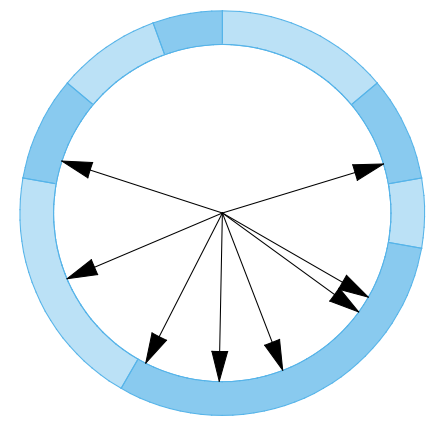
\includegraphics[width=0.2\textwidth]{figures/multinomial.png}
    \caption{Illustration of multinomial resampling with a ``resampling wheel''.\cite{parallel_resampling}}
    \label{fig:pf_resampling}
\end{figure}

\begin{algorithm}[h]
	\KwIn{population $P_{in}$, population size $n$}
	\KwOut{population $P_{out}$}
	$\ell_{max} \leftarrow \textsc{max}(\ell)$\\
	$\mathcal{W}_{sum} \leftarrow 0$\\
	$w \leftarrow$ \textsc{allocateFloats}($n$)\\
	\ForEach{particle in $P_{in}$}{
	    $\mathcal{W} \leftarrow e^{\ell - \ell_{max}}$\\
	    $\mathcal{W}_{sum} \leftarrow \mathcal{W}_{sum} + \mathcal{W}$\\
	    $w_i \leftarrow \mathcal{W}_{sum}$\\
	}
	\ForEach{$p$ in $P_{out}$}{
	    $x \leftarrow$ \textsc{random}($0$, $\mathcal{W}_{sum}$)\\
	    $i \leftarrow$ \textsc{lowerBounds}($w$, $x$)\\
	    $p \leftarrow P_{in}^{i}$\\
	}
	\Return{$P_{out}$}
	\caption{Resampling step of the particle filter as pseudocode.}
	\label{alg:pf_resampling}
\end{algorithm}

\subsection{Estimation}

To get an estimate of the hard iron vector and its error a weighted average and covariance matrix is calculated from the population of the filter. The covariance matrix can later be used to quantity the convergence of the filter.

Pseudocode can be found in Algorithm \ref{alg:pf_estimate}.

\begin{algorithm}[h]
	\KwIn{population $P$}
	\KwOut{hard iron vector $\bm{\hat{B}}_{phone}$, hard iron covariance $\bm{\hat{\Sigma}}_{phone}$, external field vector $\bm{\hat{B}}_{external}$, external field covariance $\bm{\hat{\Sigma}}_{external}$}
    $\bm{\hat{B}}_{phone} \leftarrow$ \textsc{weightedAverage($P$, $\mathcal{W}$, $\bm{B}_{phone}$)}\\
    $\bm{\hat{\Sigma}}_{phone} \leftarrow$ \textsc{weightedCovariance($P$, $\mathcal{W}$, $\bm{B}_{phone}$)}\\
    $\bm{\hat{B}}_{external} \leftarrow$ \textsc{weightedAverage($P$, $\mathcal{W}$, $\bm{B}_{external}$)}\\
    $\bm{\hat{\Sigma}}_{external} \leftarrow$ \textsc{weightedCovariance($P$, $\mathcal{W}$, $\bm{B}_{external}$)}\\
	\Return{$\bm{\hat{B}}_{phone}$, $\bm{\hat{\Sigma}}_{phone}$, $\bm{\hat{B}}_{external}$, $\bm{\hat{\Sigma}}_{external}$}
	\caption{Estimation step of the particle filter as pseudocode.}
	\label{alg:pf_estimate}
\end{algorithm}

\section{Filter routine}

The filter routine is a combination of all of the steps above in Section \ref{sec:impl_pf}. We initialize the filter with the first observation. Then we update and propagate based on time passed and newly incoming observations.

Pseudocode of the filter routine can be found in Algorithm \ref{alg:routine}.

\begin{algorithm}[h]
	\KwIn{magnetic field measurement $\bm{B}_{measure}$, orientation $\bm{q}$}
	\KwOut{calibrated magnetic field $\bm{\hat{B}}$, calibrated magnetic field covariance $\bm{\hat{\Sigma}}$}
	\If{\textsc{notInitialized()}}{
	    $P \leftarrow$ \textsc{init}($\bm{B}_{measure}$, $\bm{q}$)\\
	    \textsc{estimate}()\\
	}
	\If{\textsc{significantRotation($\bm{q}$)}}{
	    \textsc{update}($\bm{B}_{measure}$, $\bm{q}$)\\
	    $\bm{\hat{B}}_{phone}$, $\bm{\hat{\Sigma}}_{phone}$ $\leftarrow$ \textsc{estimate}()\\
	    \If{\textsc{effectiveParticles()} < \textsc{population} $\times$ \textsc{resamplingRate}}{
	        \textsc{resample}()\\
	    }
	}
	$\bm{\hat{B}} \leftarrow \bm{B}_{measure} - \bm{\hat{B}}_{phone}$\\
    $\bm{\hat{\Sigma}} \leftarrow \bm{\hat{\Sigma}}_{phone}$\\
	\Return{$\bm{\hat{B}}$, $\bm{\hat{\Sigma}}$}
	\caption{The filter routine as pseudocode.}
	\label{alg:routine}
\end{algorithm}

The filter can be parameterized with the following options.

\begin{table}[h]
    \centering
    \begin{tabular}{ | l | p{10cm} | }
    \hline
    \textbf{Parameter}       & \textbf{Description} \\ \hline
    \textsc{seed}                   & Seed for the pseudorandom number generator. \\ \hline
    \textsc{population}             & The total number of particles. \\ \hline
    \textsc{deltaTime}              & The time difference in seconds between two filter iterations. \\ \hline
    \textsc{initialVariance}        & The initial hard iron variance for the initialization procedure in $(\mu T)^2$. \\ \hline
    \textsc{driftRate}              & The hard iron calibration drift rate for the propagation procedure. \\ \hline
    \textsc{predictionVariance}     & The prediction variance for the update procedure in $(\mu T)^2$. \\ \hline
    \textsc{minimalRotation}        & Minimal rotation angle to perform an update in radians. \\ \hline
    \textsc{resamplingRate}         & Relative amount of effective particles to trigger resampling. \\ \hline
    \end{tabular}
    \caption{Parameter description of the filter.}
    \label{tbl:impl_params}
\end{table}

The filter will only update after significant rotations which is parameterized with \textsc{minimalRotation}. That has the benefit of saving \gls{cpu} consumption and ignoring noise from the orientation filter and therefore minimizing bias. Adaptive resampling is used to reduce bias and can be parameterized with \textsc{resamplingRate} and might also spare \gls{cpu} usage.

\section{Synchronization}
\label{sec:impl_synchro}

This works targets mobile devices, currently with Android and iOS. Since those are no real-time systems one has to deal with unpredictable latency and concurrency. These effects play a role while receiving data of multiple sensors possibly through multiple threads. The receiver might then observe that some events are out of order. Sequential filters rely on the causal order of the events because the state of the filter evolves with each observation and its timestamp and they cannot integrate events that are older than the state. When we combine multiple sensor streams into one result we have to be careful because of the potential difference of latency given by each stream.

This problem was solved with a synchronization step at the beginning of the pipeline. Buffers are used to hold all the incoming sensor data until it is guaranteed that all streams reached the same point in time. That guarantees that any other component behind the synchronization will only receive events that are in order and therefore does not have to deal with synchronization by itself.

\section{Down sampling}
\label{sec:impl_downsample}

As mentioned above in Section \ref{sec:impl_synchro}, we cannot rely on the properties of a real-time system. In case of Android, the requested sampling rate passed to the the sensors \gls{api} is treated as a hint and can vary greatly. Since the orientation filter relies on a constant sampling rate this problem had to be resolved by implementing a down sampling algorithm. The chosen algorithm was a rolling average.

The sampling interval was measured during evaluation and in Section \ref{sec:eval_sensor}.

\section{Orientation estimation}
\label{sec:ori_est}

We saw that this thesis highly depends on the orientation estimation of the device in Section \ref{sec:impl_pf}. Errors coming from the orientation will directly propagate into errors of the hard iron calibration. Therefore it was crucial to use a well suited algorithm to estimate the orientation with high precision. These algorithms typically use the accelerometer and the gyroscope to form an \gls{imu}.

In this thesis relies on Madgwick's \gls{imu} algorithms.\cite{madgwick} It claims to have low computational effort and higher accuracy then Kalman-based algorithms. The algorithm is illustrated in Figure \ref{fig:madgwick_imu}. The orientation filter has only a single parameter \textsc{beta} apart from the update interval which models the reliability proportion between accelerometer and gyroscope measurements.

\begin{figure}[hbt!]
    \centering
    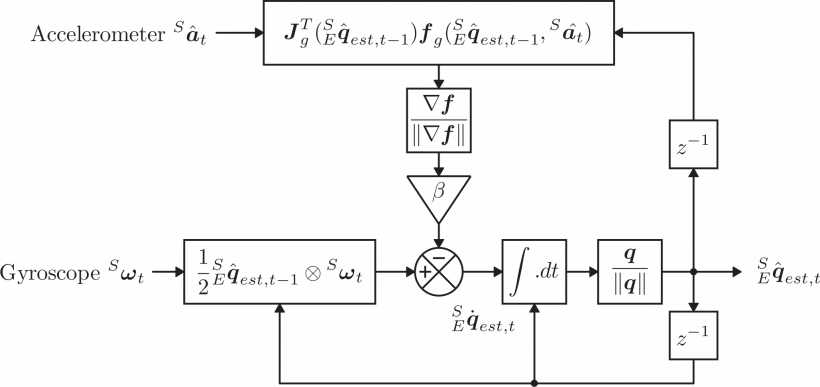
\includegraphics[width=1.0\textwidth]{figures/madgwick_imu.png}
    \caption{Block diagram representation of the orientation estimation algorithm.\cite{madgwick}}
    \label{fig:madgwick_imu}
\end{figure}

The x and y-axis in worlds coordinates will be rotated by an unknown angle along the z-axis due to missing information of the horizontal orientation. Apart from that this angle will be drifting due to errors coming from the gyroscope.

\section{Total rotation}

Since our hard iron calibration can only progress if the device is rotated we want to quantify the total rotation and use it instead of time as an axis for our plots. This was achieved by calculating the Euler axis and angle between two orientation estimates and a sum over these angles.

The quaternion $\bm{\Delta q}_i$ that transforms the previous orientation $\bm{q}_i$ to the current orientation $\bm{q}_{i+1}$ can be expressed with the following.

\[\bm{q}_{i+1} = \bm{\Delta q}_i \times \bm{q}_i\]
\[\bm{\Delta q}_i = \bm{q}_{i+1} \times \bm{q}_i^{-1}\]

The Euler angle can then be extracted with the extended Euler's formula.

\[\Delta \omega = 2 \arccos{\operatorname{Re}(\bm{\Delta q}_i)}\]

With $\operatorname{Re}(\bm{\Delta q}_i)$ as the real component of the quaternion $\bm{\Delta q}_i$.

This quantity was also used to filter for significant rotations in the hard iron calibration.

\section{Android}

Java was used to develop a small demo application that is able to read sensor data and pass it down to C++ through \gls{jni}. A webview was used to display the visualization written in JavaScript. The whole life cycle of the application is managed in Java.

The sensor \gls{api} offers a high-level interface to read sensor values by registering to a specific sensor type, like accelerometer, providing a sampling rate, and a callback for incoming data.\cite{android_sdk_sensormanager}. The \gls{api} is presenting calibrated and uncalibrated sensor readings in the same way and is distinguishing between them by identifier. \textsc{TYPE\_MAGNETIC\_FIELD} can be used to read the system calibrated magnetic field and \textsc{TYPE\_MAGNETIC\_FIELD\_UNCALIBRATED} for the uncalibrated magnetic field, which is required for this thesis.

From experience we know that the sensor \gls{api} will not sample the sensors a constant rate. Since a constant sampling rate is a requirement for the orientation filter this problem had to be resolved. This is discussed in Section \ref{sec:impl_downsample}.

A screenshot of the application is shown in Figure \ref{fig:app}.

\begin{figure}[hbt!]
    \centering
    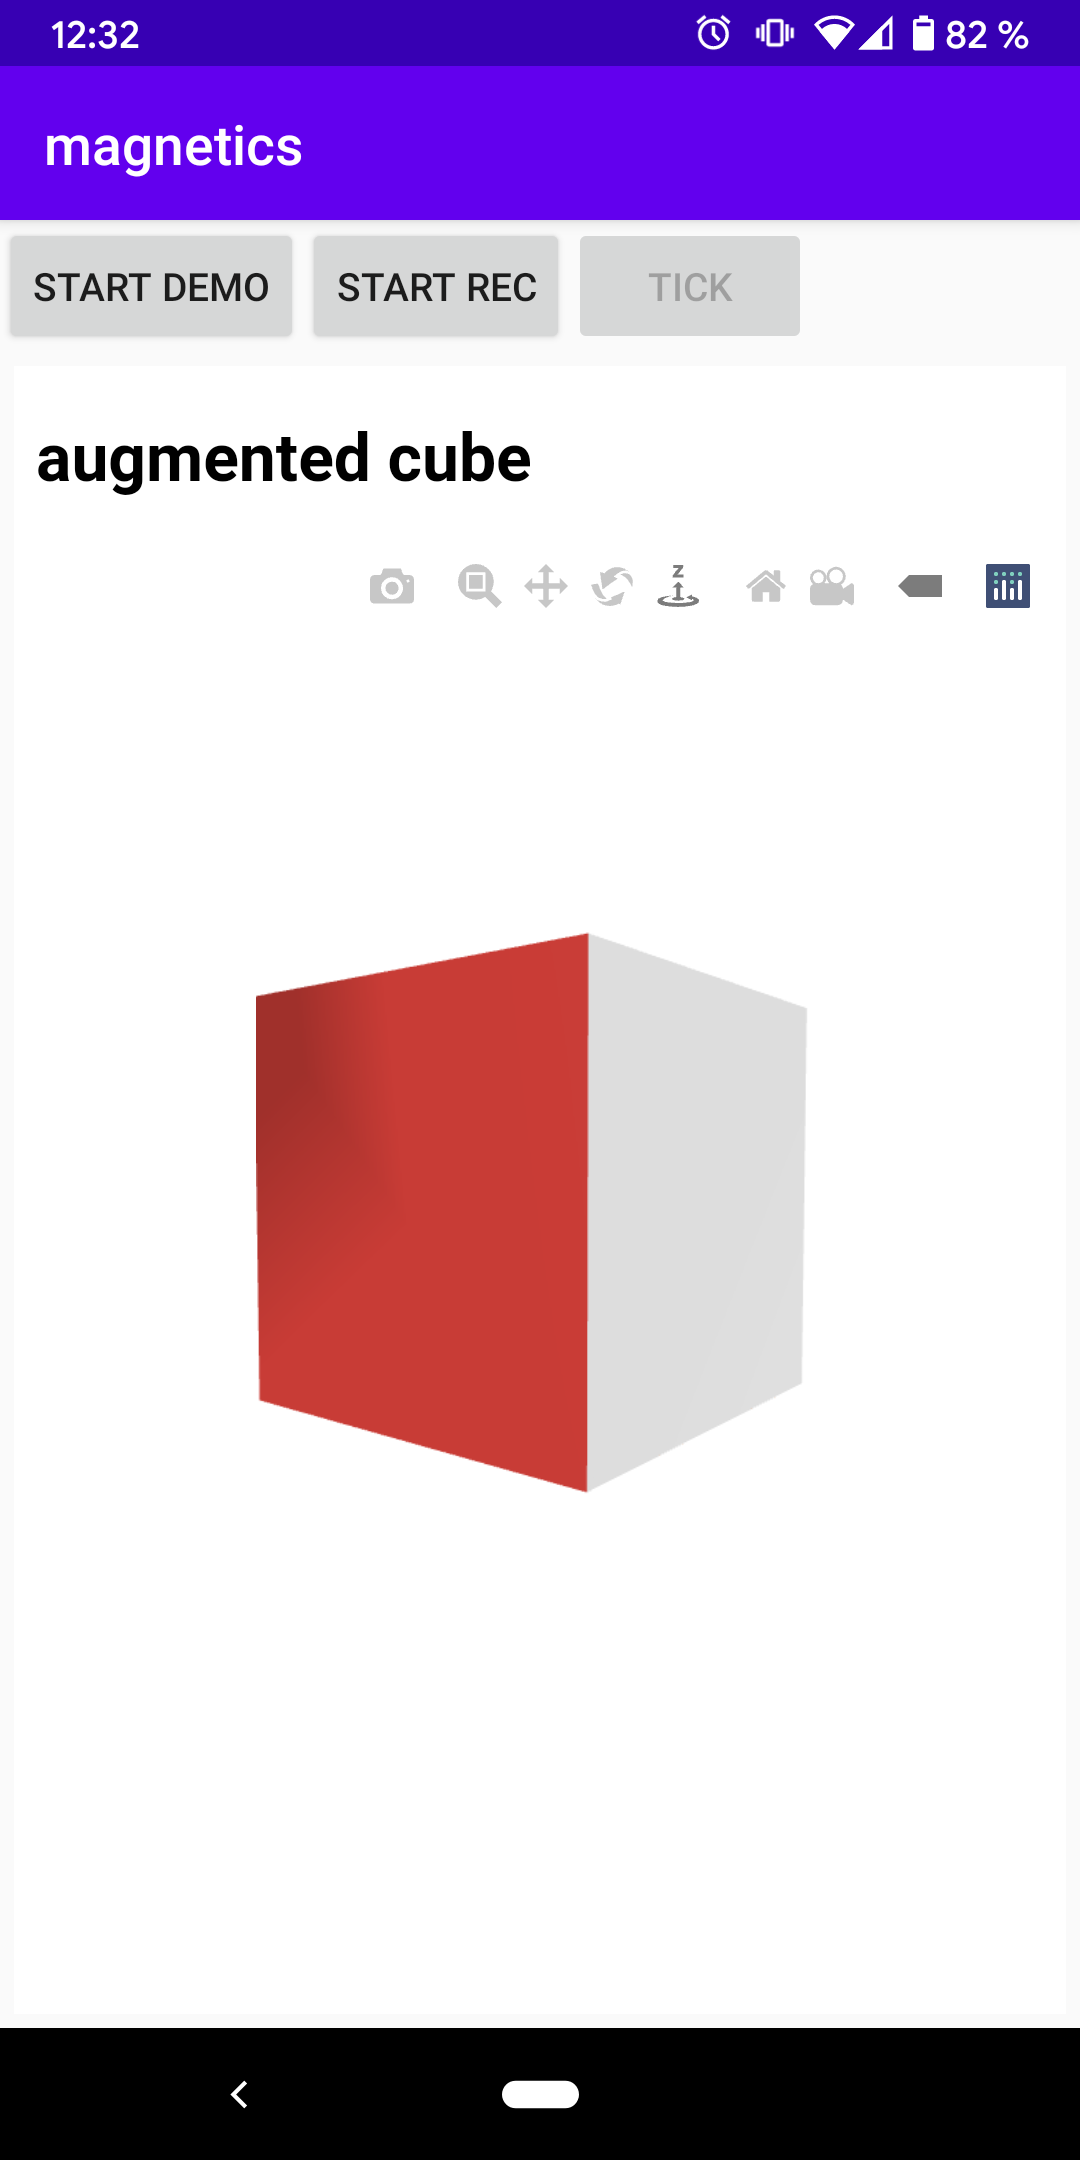
\includegraphics[width=0.4\textwidth]{figures/app.png}
    \caption{Screenshot for the Android application.}
    \label{fig:app}
\end{figure}

\section{Visualization}

One goal for the visualization was to build it platform independent to have the same code for desktop and mobile. This is very beneficial because the visualization can be driven by simulated and real-time sensor data.

The initial idea was to use OpenGL ES for that purpose which is supported by Android and on modern desktop \gls{os}. One visualization idea was a three-dimensional scatter plot for the acquired magnetic field sensor data to build up intuition. OpenGL is executed by the \gls{gpu} so there was no performance concerns about that.

Since progress was rather slow and the implementation effort was growing quickly the desire for an alternative was rising. Plotly with JavaScript seemed to be a good solution for platform independence and it also claimed to have good performance with WebGL backend for 3D plots. The HTML and JavaScript code was stored as an asset along the demo application and displayed with a webview on Android. On the desktop it is sufficient to use any modern browser to run the visualization.
